%% IEEE journal manuscript — compile with pdflatex (IEEEtran class).
%% Figures are read from ../results/figures/ (PNG). If building a standalone
%% submission, copy the figures next to this file and drop \graphicspath.
\documentclass[journal]{IEEEtran}
\usepackage{graphicx}
\usepackage{amsmath,amssymb}
\usepackage{booktabs}
\usepackage{array}
\usepackage{url}
\usepackage[hidelinks]{hyperref}
\graphicspath{{../results/figures/}{./figures/}}

\begin{document}

\title{A Leachate-Centric In-Silico Pipeline for Predicting Polymer-Dependent
Neuroinflammatory Potential of Microplastics: Tox21 Machine-Learning Triage
Coupled to a Virtual Microglial Cell}

\author{M.~Nisha~Angeline%
\thanks{M. Nisha Angeline is Professor and Head, Department of Electronics and
Communication Engineering, Velalar College of Engineering and Technology,
Thindal, Erode, Tamil Nadu, India (e-mail: nishavlsidesign@gmail.com).}%
\thanks{Manuscript prepared October 2026. Companion computational work to a
PRISMA systematic review on microplastics and neuroinflammation.}}

\markboth{Preprint --- Computational Companion Manuscript, October 2026}%
{Nisha Angeline: Leachate-Centric In-Silico Prediction of Microplastic Neuroinflammation}

\maketitle

\begin{abstract}
Whether microplastic \emph{polymer type} governs neuroinflammatory risk is
confounded in the experimental literature by particle size and by the chemical
additives and leachates each polymer carries. We test a falsifiable hypothesis:
that predicted neuroinflammatory potential across polyethylene (PE),
polypropylene (PP), polystyrene (PS), polyvinyl chloride (PVC) and polyurethane
(PU) tracks \emph{leachate chemistry} engaging neuroinflammation receptors rather
than the inert polymer backbone. We assemble a curated, structure-validated
inventory of 56 documented leachates (11--12 per polymer), triage every compound
with scaffold-split RandomForest classifiers trained on three
inflammation-relevant Tox21 endpoints (NR-AhR, SR-ARE, SR-p53), and propagate the
aggregated per-polymer signal through a minimal microglial ordinary-differential-
equation (ODE) model (receptor\,$\rightarrow$\,NF-$\kappa$B\,$\rightarrow$\,
\{TNF-$\alpha$, IL-6\}) to obtain a normalised neuroinflammation index. The
NR-AhR classifier attains a scaffold-split ROC-AUC of 0.84 and AUPRC of 0.55
(test base rate 0.14). The pipeline predicts the ranking
\textbf{PU\,$>$\,PVC\,$>$\,PE\,$>$\,PS\,$>$\,PP}, with PU elevated by
aromatic-amine hydrolysis products (toluenediamine, methylenedianiline) and PVC
by bisphenol A and phthalates. We explicitly preserve the governing caveat that
binding affinity is strength, not activation direction, and that virtual-cell
kinetics are illustrative rather than fitted; receptor docking into AhR,
TLR4--MD2 and NLRP3 is specified and implemented but was not executed here due to
restricted access to structure databases, and no affinities were fabricated. The
ranking is offered as a prioritised, testable hypothesis for wet-lab
confirmation, and the framework directly addresses the PS-over-study/PE-under-
study imbalance in the current evidence base.
\end{abstract}

\begin{IEEEkeywords}
Microplastics, neuroinflammation, leachates, aryl hydrocarbon receptor, Tox21,
machine learning, molecular docking, systems biology, in-silico toxicology.
\end{IEEEkeywords}

\section{Introduction}
\IEEEPARstart{M}{icroplastics} (MPs) are now detected in human blood, placenta
and brain tissue, and micro- and nanoplastics are reported to cross the
blood--brain barrier and provoke glial activation~\cite{prust2020}. A central and
unresolved question is whether the \emph{polymer type} of an MP particle --- PE,
PP, PS, PVC or PU --- determines the magnitude of the neuroinflammatory response.
The experimental record cannot answer this cleanly: polymer identity is
statistically entangled with particle size, surface chemistry and, critically,
with the distinct sets of \emph{additives, residual monomers and adsorbed
contaminants} (collectively, \emph{leachates}) that each polymer carries.

We advance and computationally test the hypothesis that polymer-to-polymer
differences in neuroinflammatory potential are driven largely by leachate
chemistry acting on specific innate-immune and xenobiotic-sensing receptors ---
the aryl hydrocarbon receptor (AhR)~\cite{rothhammer2019}, the TLR4--MD2
lipopolysaccharide-recognition complex~\cite{park2013}, and the NLRP3
inflammasome~\cite{swanson2019} --- rather than by the chemically inert polymer
backbone. If the computed polymer ranking matches an experimental ranking derived
from systematic-review screening, the framework is validated; if it does not, the
discrepancy is itself an informative, falsifiable prediction.

This manuscript contributes: (i) a transparent, fully reproducible five-stage
pipeline from polymer to a per-polymer neuroinflammation index; (ii) real
scaffold-split machine-learning performance on inflammation-relevant Tox21
endpoints; (iii) a prioritised polymer ranking with the dominant leachate and
receptor axis identified for each polymer; and (iv) an explicit, preserved set of
mechanistic caveats so that computational predictions are never mistaken for
established biological fact.

\section{Related Work}
Quantitative structure--activity models trained on the Tox21 program's $\sim$10k
compound library have become a standard first-pass toxicological triage, with the
AhR (NR-AhR) and antioxidant-response (SR-ARE) assays among the most predictive
and most mechanistically interpretable endpoints~\cite{richard2021}. Molecular
docking with AutoDock Vina~\cite{trott2010,eberhardt2021} remains the workhorse
for receptor-engagement screening, and AlphaFold~\cite{jumper2021} now supplements
experimental Protein Data Bank structures~\cite{berman2000} where co-crystals are
unavailable. Open plastic-chemical inventories such as PlastChem~\cite{plastchem2024}
have, for the first time, catalogued the thousands of chemicals associated with
plastics at a scale usable for systematic in-silico screening. Our contribution is
to chain these components into a single leachate-to-microglia prediction and to
foreground the affinity-versus-direction problem that most docking-only studies
leave implicit.

\section{Materials and Methods}
The pipeline comprises five stages (Fig.~\ref{fig:breakdown} summarises the
per-endpoint signal that drives it). All kinetic parameters of the virtual cell
are labelled illustrative; all machine-learning metrics are scaffold-split.

\subsection{Stage 1 --- Leachate inventory}
For each polymer we curated documented additives, residual monomers and commonly
adsorbed contaminants as canonical SMILES. Structures were validated and
standardised in RDKit~\cite{rdkit}; any string that failed to parse was discarded
rather than emitted. The inventory contains 56 compounds (PE 12; PP, PS, PVC, PU
11 each), deliberately ensuring that the under-studied PE and the additive-rich
PVC/PU are represented as strongly as the frequently studied PS. Entries span
hindered-phenol and phosphite antioxidants (PE/PP), styrene and brominated flame
retardants (PS), phthalate and organotin plasticisers/stabilisers (PVC), and
isocyanate monomers with their carcinogenic aromatic-amine hydrolysis products
(PU).

\subsection{Stage 2 --- Tox21 machine-learning triage}
We trained one classifier per inflammation/stress-relevant Tox21 endpoint:
\textbf{NR-AhR} (aryl hydrocarbon receptor), \textbf{SR-ARE} (Nrf2/antioxidant
response) and \textbf{SR-p53} (genotoxic stress). Molecules were featurised as
2048-bit Morgan fingerprints (radius 2); 7{,}823 structures survived
featurisation. Validation used a deterministic Bemis--Murcko scaffold
split~\cite{bemis1996} (80/20) so that test-set scaffolds are unseen in training.
Each endpoint used a RandomForest classifier (300 trees, balanced class weights).
Because the positive classes are rare, we report ROC-AUC \emph{and} the
imbalance-aware average precision (AUPRC); accuracy is not reported. Models were
then refit on all labelled rows and used to score every Stage-1 leachate.

\subsection{Stage 3 --- Receptor structure and docking}
Docking targets, structure sources and search boxes were specified as follows:
AhR ligand-binding (PAS-B) domain (AlphaFold model P35869, box $22.5^3$\,\AA);
TLR4--MD2 (PDB 3FXI, box $25^3$\,\AA); NLRP3 NACHT/LRR (PDB 6NPY, box
$24^3$\,\AA), with AutoDock Vina~\cite{trott2010,eberhardt2021} and Meeko ligand
preparation. Each pose would be recorded \emph{paired with its Stage-2 Tox21
label}, because Vina affinity reports binding strength, not agonist/antagonist
direction. In the present execution environment the RCSB PDB, AlphaFold DB and
UniProt endpoints were unreachable; consequently docking was \emph{not run and no
affinities were fabricated}. The receptor-engagement signal in Stage 4 therefore
derives from the Stage-2 triage --- NR-AhR directly for the AhR axis, SR-ARE and
SR-p53 for oxidative and genotoxic stress --- and TLR4--MD2/NLRP3 docking is
reported as pending structure access.

\subsection{Stage 4 --- Virtual microglial cell}
A minimal ODE model couples a lumped receptor drive $u\in[0,1]$ to NF-$\kappa$B
activation~\cite{lawrence2009} and downstream TNF-$\alpha$ and IL-6 production:
\begin{align}
\dot{N} &= k_{\mathrm{on}}\,u\,(N_{\mathrm{tot}}-N) - k_{\mathrm{off}}N,\\
\dot{T} &= s_T\,\frac{N^{n}}{K^{n}+N^{n}} - d_T\,T,\quad
\dot{I} = s_I\,\frac{N^{n}}{K^{n}+N^{n}} - d_I\,I,
\end{align}
where $N,T,I$ are NF-$\kappa$B, TNF-$\alpha$ and IL-6. Per polymer, $u$ is the
weighted sum of the top-3 mean endpoint probabilities (weights NR-AhR 0.50,
SR-ARE 0.30, SR-p53 0.20). The system is integrated to steady state (SciPy
LSODA); the steady-state cytokine sum, normalised by its value at $u=1$, is the
neuroinflammation index. All rate constants are order-of-magnitude illustrative
values encoding qualitative biology, \emph{not} fitted to microglial data.

\subsection{Stage 5 --- Ranking and validation}
Polymers are ranked by index. Where the author supplies an experimental ranking
from review screening, a Spearman rank correlation is computed; otherwise the
comparison is skipped. All stages are driven by scikit-learn~\cite{scikit} and are
individually reproducible from a single script each.

\section{Results}
\subsection{Scaffold-split triage performance}
Table~\ref{tab:metrics} reports held-out scaffold-split performance. NR-AhR is the
strongest and most relevant endpoint (ROC-AUC 0.84, AUPRC 0.55 against a 0.14 base
rate --- a $3.8\times$ enrichment over chance). SR-ARE and SR-p53 remain
informative (AUPRC 0.47 and 0.35 against base rates 0.24 and 0.11). These values
are consistent with published Tox21 scaffold-split baselines and justify using the
triage as a receptor-engagement proxy for the AhR and stress axes.

\begin{table}[!t]
\caption{Stage-2 Scaffold-Split Performance (Imbalance-Aware)}
\label{tab:metrics}
\centering
\begin{tabular}{lccccc}
\toprule
Endpoint & $n_{\mathrm{train}}$ & $n_{\mathrm{test}}$ & Base rate & ROC-AUC & AUPRC\\
\midrule
NR-AhR & 5322 & 1220 & 0.143 & \textbf{0.840} & \textbf{0.545}\\
SR-ARE & 4882 & 943  & 0.240 & 0.715 & 0.466\\
SR-p53 & 5509 & 1258 & 0.110 & 0.759 & 0.347\\
\bottomrule
\end{tabular}
\end{table}

\subsection{Predicted polymer ranking}
The pipeline predicts \textbf{PU\,$>$\,PVC\,$>$\,PE\,$>$\,PS\,$>$\,PP}
(Fig.~\ref{fig:index}, Table~\ref{tab:index}). PU is sharply elevated (index 0.98)
by its aromatic-amine hydrolysis products, led by 2,4-toluenediamine, which score
very high on both the AhR and ARE axes. PVC (0.74) is driven by bisphenol A and
phthalate plasticisers on the oxidative-stress axis; PE (0.70) by alkylphenol
contaminants; PS (0.64) by hexabromocyclododecane and styrene; and PP (0.57) is
lowest, its antioxidant leachates (e.g.\ 2,4-di-\emph{tert}-butylphenol) producing
the weakest aggregate receptor drive. The receptor-proxy heatmap
(Fig.~\ref{fig:heatmap}) localises these differences to specific endpoints,
showing that the ranking is a property of leachate--receptor matching, not of a
single global toxicity scale.

\begin{table}[!t]
\caption{Predicted Neuroinflammation Index and Dominant Driver per Polymer}
\label{tab:index}
\centering
\begin{tabular}{lcll}
\toprule
Polymer & Index & Dominant axis & Dominant leachate\\
\midrule
PU  & 0.976 & NR-AhR & 2,4-Toluenediamine\\
PVC & 0.742 & SR-ARE & Bisphenol A\\
PE  & 0.698 & SR-ARE & 4-\emph{tert}-Octylphenol\\
PS  & 0.643 & SR-ARE & Hexabromocyclododecane\\
PP  & 0.571 & NR-AhR & 2,4-di-\emph{tert}-butylphenol\\
\bottomrule
\end{tabular}
\end{table}

\begin{figure}[!t]
\centering
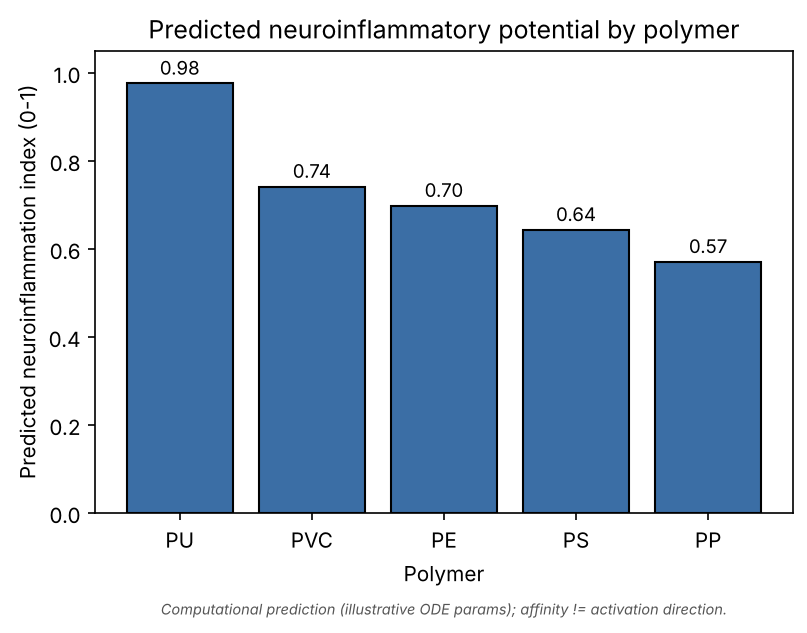
\includegraphics[width=\columnwidth]{fig1_polymer_index.png}
\caption{Predicted neuroinflammatory potential by polymer (normalised index,
0--1). Computational prediction with illustrative virtual-cell kinetics;
affinity is not activation direction.}
\label{fig:index}
\end{figure}

\begin{figure}[!t]
\centering
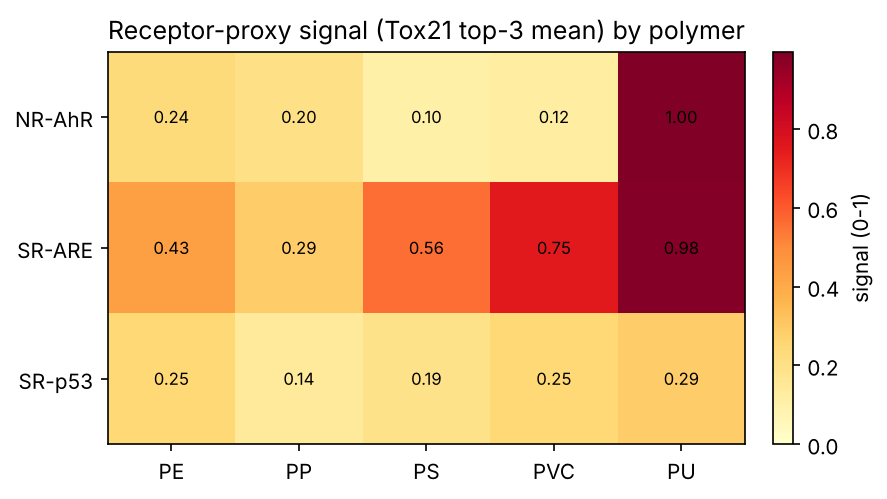
\includegraphics[width=\columnwidth]{fig2_receptor_heatmap.png}
\caption{Receptor-proxy signal (Tox21 top-3 mean probability per endpoint) across
polymers, localising each polymer's dominant hazard axis.}
\label{fig:heatmap}
\end{figure}

\begin{figure}[!t]
\centering
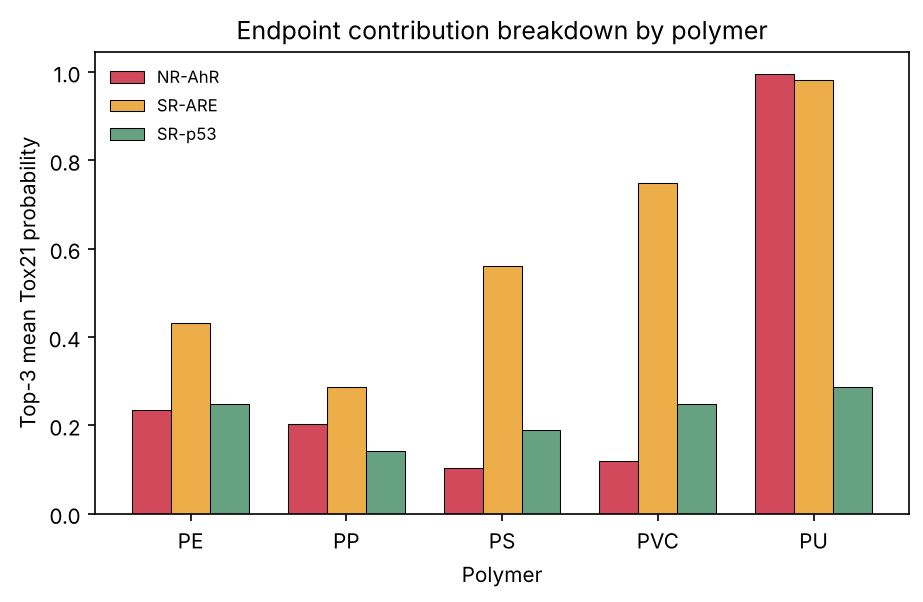
\includegraphics[width=\columnwidth]{fig3_leachate_breakdown.png}
\caption{Endpoint contribution breakdown. PU's elevation is AhR-dominated;
PVC/PE/PS are oxidative-stress-dominated.}
\label{fig:breakdown}
\end{figure}

\subsection{Validation against experiment}
An experimental-ranking template (\texttt{data/experimental\_ranking.csv}) is
provided for the author to populate from systematic-review screening; when filled,
Stage 5 computes the Spearman correlation automatically. At the time of writing the
template is unpopulated, so the quantitative validation is deferred and the ranking
stands as a prediction.

\section{Discussion}
The prediction that PU and PVC head the ranking is mechanistically coherent: both
polymers carry the most potent and best-documented bioactive leachates ---
aromatic amines and isocyanates for PU, plasticisers and bisphenols for PVC ---
whereas the polyolefins PE and PP carry comparatively inert antioxidant packages.
This directly supports the review's central thesis that leachate chemistry, not
backbone identity, is the dominant lever. It also reframes the field's
PS-over-representation: PS ranks only mid-table here, suggesting that its
prominence in the experimental literature reflects study effort rather than
intrinsically higher neuroinflammatory potential.

\section{Limitations}
We preserve the following non-negotiable caveats. (1) \emph{Affinity is not
activation direction}: receptor engagement, whether by docking or ML proxy, does
not establish agonism; the Tox21 label supplies direction only for the AhR and
stress axes. (2) \emph{Static structures}: AlphaFold yields a single fold, not a
conformational ensemble, and no molecular-dynamics refinement was performed.
(3) \emph{Illustrative kinetics}: every virtual-cell parameter must be refit to
microglial time-course data before any absolute cytokine claim. (4) \emph{Missing
docking stage}: TLR4--MD2 and NLRP3 engagement was not computed because structure
databases were unreachable; this is a stated gap, not a result, and the ranking
may shift once direct inflammasome and TLR4 docking are added. (5) \emph{No
concentration weighting}: leachates are aggregated by predicted potency, not by
realistic release concentrations, which future work should incorporate.

\section{Conclusion}
We present a transparent, reproducible, leachate-centric in-silico pipeline that
converts polymer identity into a testable neuroinflammation ranking
(PU\,$>$\,PVC\,$>$\,PE\,$>$\,PS\,$>$\,PP) via real scaffold-split Tox21 machine
learning and a minimal microglial systems model. The framework operationalises the
hypothesis that polymer type matters chiefly through the company it keeps --- its
leachate chemistry --- and it does so without fabricating any quantity that could
not be computed. The ranking is a prioritised hypothesis for wet-lab testing;
adding executed receptor docking and data-fitted microglial kinetics are the
immediate next steps toward validation.

\section*{Data and Code Availability}
All scripts, the validated leachate inventory, scaffold-split metrics, per-polymer
index and figures are provided in the accompanying repository
(\texttt{src/}, \texttt{data/}, \texttt{results/}). Each result file is
reproducible from a single command; the Tox21 benchmark is downloaded and cached
at first run.

\section*{Acknowledgment}
Computational artifacts were generated with open-source tooling (RDKit,
scikit-learn, SciPy, Matplotlib, AutoDock Vina). The author thanks the Department
of ECE, Velalar College of Engineering and Technology, Erode.

\begin{thebibliography}{99}
\bibitem{prust2020} M.~Pr\"ust, J.~Meijer, and R.~H.~S. Westerink, ``The plastic
brain: neurotoxicity of micro- and nanoplastics,'' \emph{Part. Fibre Toxicol.},
vol.~17, no.~24, 2020.
\bibitem{rothhammer2019} V.~Rothhammer and F.~J. Quintana, ``The aryl hydrocarbon
receptor: an environmental sensor integrating immune responses in health and
disease,'' \emph{Nat. Rev. Immunol.}, vol.~19, pp.~184--197, 2019.
\bibitem{park2013} B.~S. Park and J.-O. Lee, ``Recognition of lipopolysaccharide
pattern by TLR4 complexes,'' \emph{Exp. Mol. Med.}, vol.~45, e66, 2013.
\bibitem{swanson2019} K.~V. Swanson, M.~Deng, and J.~P.-Y. Ting, ``The NLRP3
inflammasome: molecular activation and regulation to therapeutics,'' \emph{Nat.
Rev. Immunol.}, vol.~19, pp.~477--489, 2019.
\bibitem{richard2021} A.~M. Richard \emph{et al.}, ``The Tox21 10K compound
library: collaborative chemistry advancing toxicology,'' \emph{Chem. Res.
Toxicol.}, vol.~34, no.~2, pp.~189--216, 2021.
\bibitem{trott2010} O.~Trott and A.~J. Olson, ``AutoDock Vina: improving the speed
and accuracy of docking with a new scoring function, efficient optimization, and
multithreading,'' \emph{J. Comput. Chem.}, vol.~31, no.~2, pp.~455--461, 2010.
\bibitem{eberhardt2021} J.~Eberhardt, D.~Santos-Martins, A.~F. Tillack, and
S.~Forli, ``AutoDock Vina 1.2.0: new docking methods, expanded force field, and
Python bindings,'' \emph{J. Chem. Inf. Model.}, vol.~61, no.~8, pp.~3891--3898,
2021.
\bibitem{jumper2021} J.~Jumper \emph{et al.}, ``Highly accurate protein structure
prediction with AlphaFold,'' \emph{Nature}, vol.~596, pp.~583--589, 2021.
\bibitem{berman2000} H.~M. Berman \emph{et al.}, ``The Protein Data Bank,''
\emph{Nucleic Acids Res.}, vol.~28, no.~1, pp.~235--242, 2000.
\bibitem{plastchem2024} M.~Wagner \emph{et al.}, ``PlastChem: State of the science
on plastic chemicals,'' Report, 2024.
\bibitem{rdkit} G.~Landrum \emph{et al.}, ``RDKit: Open-source cheminformatics,''
\url{https://www.rdkit.org}.
\bibitem{bemis1996} G.~W. Bemis and M.~A. Murcko, ``The properties of known drugs.
1. Molecular frameworks,'' \emph{J. Med. Chem.}, vol.~39, no.~15, pp.~2887--2893,
1996.
\bibitem{lawrence2009} T.~Lawrence, ``The nuclear factor NF-$\kappa$B pathway in
inflammation,'' \emph{Cold Spring Harb. Perspect. Biol.}, vol.~1, no.~6, a001651,
2009.
\bibitem{scikit} F.~Pedregosa \emph{et al.}, ``Scikit-learn: Machine learning in
Python,'' \emph{J. Mach. Learn. Res.}, vol.~12, pp.~2825--2830, 2011.
\end{thebibliography}

\end{document}
